%!TEX root = ../main.tex %
% !TeX spellcheck = en_US

%%%%%%%  INTRODUCTION  %%%%%%%%%

\section{Introduction to Excitons in 2D Materials}
%%%%%%%%%%%%%%%%%%%%%%%%%%%%%%%%%%%%%%%%%%%%%%%%%%%%%%%%%%%%%%%%%%%%

% \begin{frame}{Optical Excitations in Matter}
%     \centering
%     
\begin{tikzpicture}[mindmap, grow cyclic, every node/.style=concept, concept color=blue!40!white,
    level 1/.append style={level distance=3.5cm,sibling angle=120},
    level 2/.append style={level distance=2.8cm,sibling angle=45},
    level 3/.append style={level distance=2cm,sibling angle=40},
    every annotation/.style={fill=red!20}]
    \tikzset{every node/.append style={scale=0.8}}
\node [concept,scale=1.0] (center) {\Large Solid Materials}

    child [concept color = violet!60!white,grow=-150] {
        node[alt=<{2}>{circular glow={fill=brass}}{}] (metals) {Metals} 
            child[visible on=<3->,grow=120] { node[alt=<{3}>{circular glow={fill=brass}}{}] {Free charges}}
            child[visible on=<4->,grow=180] { node[alt=<{4}>{circular glow={fill=brass}}{}] {Conducting}}
            child[visible on=<5->,grow=-120] { node[alt=<{5}>{circular glow={fill=brass}}{}] {Plasmons}}}
    child [concept color = red!60!white,grow=-30] { 
        node[alt=<{6}>{circular glow={fill=brass}}{}] (dielectrics) {Dielectric}
            child[visible on=<7->,grow=60] { node[alt=<{7}>{circular glow={fill=brass}}{}] {Bound charges}}
            child[visible on=<8->,grow=0] { node[alt=<{8}>{circular glow={fill=brass}}{}] {Insulating}}
            child[visible on=<9->,grow=-60] { node[alt=<{9}>{circular glow={fill=brass}}{}] {Excitons}}
    };

    %\path (center) to[circle connection bar switch color=from (blue!40!white) to (violet!60!white)] (metals);
    % \node [right,text width=5.2cm, minimum width = 5.2cm,visible on=<3->] at (metals.south west)
    %     {Free charge };
    % \path (center) to[circle connection bar switch color=from (blue!40!white) to (red!60!white)] (dielectrics);
    % \node [annotation,right,text width=8.cm, minimum width = 8.cm,visible on=<5->] at (dielectrics.south east)
    %     {Excitons};

\end{tikzpicture}

% \end{frame}

\begin{frame}{Optical Excitations in Matter}
   \centering
    



\tikzset{every picture/.style={line width=0.75pt}} %set default line width to 0.75pt        

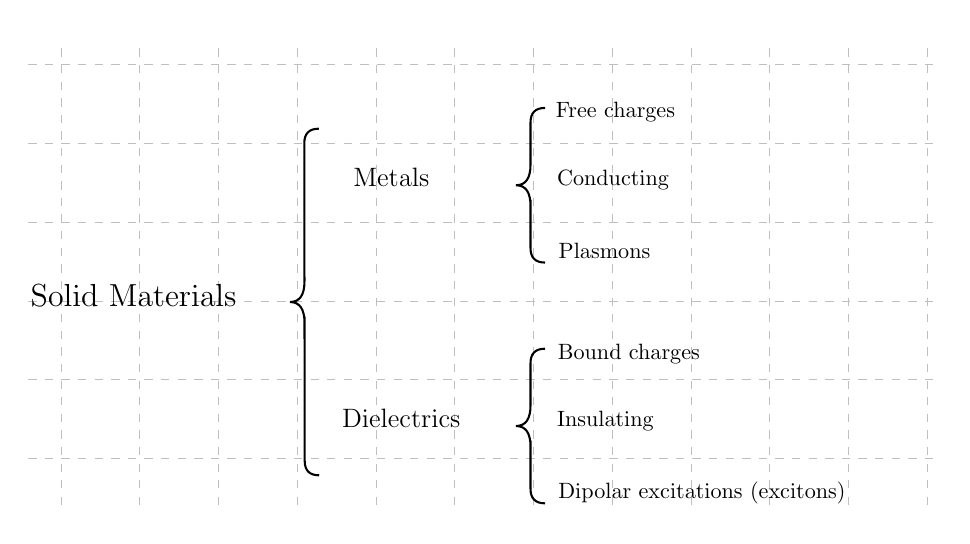
\begin{tikzpicture}[x=0.75pt,y=0.75pt,yscale=-1,xscale=1,remember picture]
%uncomment if require: \path (0,300); %set diagram left start at 0, and has height of 300
\draw[lightgray,thin,dashed] (60,30)  grid  (500,250);
\useasboundingbox (60,20) rectangle (500,255);

\begin{scope}[yshift={9.5}]
    %\fill[fill=blue!10] (60,30) rectangle (500,250);
%Shape: Brace [id:dp45369403742662895] 
\draw<2->   (200,56) .. controls (195.33,56.01) and (193,58.34) .. (193.01,63.01) -- (193.09,129.51) .. controls (193.1,136.18) and (190.77,139.51) .. (186.1,139.52) .. controls (190.77,139.51) and (193.1,142.84) .. (193.11,149.51)(193.11,146.51) -- (193.2,216.01) .. controls (193.2,220.68) and (195.53,223.01) .. (200.2,223) ;
%Shape: Brace [id:dp9306672772670488] 
\draw<5->   (309,46) .. controls (304.33,46) and (302,48.33) .. (302,53) -- (302,73.25) .. controls (302,79.92) and (299.67,83.25) .. (295,83.25) .. controls (299.67,83.25) and (302,86.58) .. (302,93.25)(302,90.25) -- (302,113.5) .. controls (302,118.17) and (304.33,120.5) .. (309,120.5) ;
%Shape: Brace [id:dp8400849826669508] 
\draw<9->   (309,162) .. controls (304.33,162) and (302,164.33) .. (302,169) -- (302,189.25) .. controls (302,195.92) and (299.67,199.25) .. (295,199.25) .. controls (299.67,199.25) and (302,202.58) .. (302,209.25)(302,206.25) -- (302,229.5) .. controls (302,234.17) and (304.33,236.5) .. (309,236.5) ;

% \draw (200.,87.) -- (340,87.);
% \draw (200.,203.0) -- (340,203.0);

% Text Node
\draw<1-> (60,130) node [anchor=north west][inner sep=0.75pt]  [font=\Large] [align=left] {Solid Materials};
% Text Node
\draw<3-> (215.4,74.) node [anchor=north west][inner sep=0.75pt]  [font=\large] [align=left] {Metals};
% Text Node
\draw<4-> (210,190.0) node [anchor=north west][inner sep=0.75pt]  [font=\large] [align=left] {Dielectrics};
% Text Node
\draw<6-> (313,42.0) node [anchor=north west][inner sep=0.75pt]   [align=left] {Free charges};
% Text Node
\draw<7-> (313.6,75.) node [anchor=north west][inner sep=0.75pt]   [align=left] {Conducting};
% Text Node
\draw<8-> (314.4,110) node [anchor=north west][inner sep=0.75pt]   [align=left] {Plasmons};
% Text Node
\draw<10-> (314,158.6) node [anchor=north west][inner sep=0.75pt]   [align=left] {Bound charges};
% Text Node
\draw<11-> (313.6,191.0) node [anchor=north west][inner sep=0.75pt]   [align=left] {Insulating};
% Text Node
\draw<12-> (314.2,225.0) node [anchor=north west][inner sep=0.75pt]   [align=left] {Dipolar excitations (excitons)};
\end{scope}

\end{tikzpicture}
\end{frame}

\subsection{Context}

\begin{frame}{Excitons in photonics}

\begin{textblock*}{5.0cm}(0.2cm,1.2cm)
Relevant for:
\end{textblock*}

\begin{textblock*}{5.0cm}(0.2cm,2.0cm)
    \,\,\,\,\,\,\, {\color<2>{red} Light--matter interactions}
    \begin{figure}
        \includegraphics[scale=0.3]{Figures/light_matter.png}
    \end{figure}
    \,\,\,\,\,\,\, \small J. Shang et al. - \textit{ACS Photonics} \\ 
    \hspace{1.4cm} \textbf{10} 7 (2023)
    % mainly in 2D dimensions, constitute a playground to study light−matter interactions, many-body effects and their applications in photonics
\end{textblock*}

\begin{textblock*}{5.0cm}(5.2cm,2.0cm)
    \,\,\,\,\,\,\, {\color<3>{red}Quantum Light Sources}
    \begin{figure}
        \includegraphics[scale=0.25]{Figures/photon_emission.png}
    \end{figure}
    \,\,\,\,\,\,\, \small S. Fiedler et al. - \textit{2D Mater.} \\ 
    \hspace{1.6cm} \textbf{10} 021002 (2023)
    % tunable photon emission from 2D semiconductors
\end{textblock*}

\begin{textblock*}{5.0cm}(10.5cm,2.0cm)
    \,\,\,\,\,\,\,\,\,\,\, {\color<4>{red}Valleytronics}
    \begin{figure}
        \includegraphics[scale=0.3]{Figures/communications.png}
    \end{figure}
    \,\,\,\,\,\,\, \small Yi Zhu et al. - \textit{Nano Letters} \\
    \hspace{1.8cm} \textbf{25} 21 (2025)
    % improve optical communication systems
\end{textblock*}


\end{frame}

\begin{frame}{Excitons in two-dimensional materials}
        \begin{columns}[T]

            \column{.5\linewidth}
            \onslide<1->{
                \textbf{For a typical 3D material (e.g., GaAs)}
                \begin{equation*}
                    \begin{aligned}
                        E_{b,n} &= - \frac{R^*}{n^2} \\
                        R^*     &= \frac{2 \mu_{eh}^2 e^4}{\hbar^2 (8 \pi \varepsilon \varepsilon_0)^2}
                    \end{aligned}                   
                \end{equation*}
            }
            \column{.5\linewidth}
            \onslide<2->{
                \textbf{\,\,\,\,\, But for a 2D (insulating) material}

                \begin{figure}
                    \centering
                    \includegraphics[scale=1.]{Figures/hBN_permittivity.pdf}
                \end{figure}
            }
            
        \end{columns}


        \begin{columns}[T]

            \column{.6\linewidth}
            \begin{textblock*}{10.0cm}(0.cm,5.0cm)            
                \only<4->{
                    \vspace{-0.5cm}
                    \hspace{-0.5cm}
                    \begin{figure}
                        \includegraphics[scale=0.4]{Figures/Exciton_Series_b}
                    \end{figure}
                    \vspace{-0.4cm}
                    A. Chernikov et al. - \textit{Phys. Rev. Lett.} \textbf{113} 076802 (2014)
                }
            \end{textblock*}
%            \only<5>{
%                \begin{itemize}
%                    \item "Theoretical Methods for Excitonic Physics in 2D Materials", Maurício et al. Phys. Status Solidi B, 259: 2200097, 2022 \small (tutorial for exciton calculation methods)
%                    \item "Diele. screening in 2D insu.: Implications for excitonic and impurity states in graphane", Cudazzo et al., Phys. Rev. B \textbf{84}, 085406, 2011 \small (classical model for $\varepsilon(q)$)
%                \end{itemize}
%            }
            
            \column{.4\linewidth}
            \onslide<3->{
                \begin{itemize}
                    \item Excitonic series $\neq$ Rydberg series
                    \item Dielectric "constant" $\varepsilon = \lim_{q \to 0} \lim_{\omega \to 0} \varepsilon (q, \omega) = 1$
                    \item $\varepsilon (q)$ highly dependent on $q$ (non-locality)
                \end{itemize}
            }
            

        \end{columns}

\end{frame}

\subsection{Motivation}
%%%%%%%%%%%%%%%%%%%%%%%%%%%%%%%%%%%%%%%%%%%%%%%%%%%%%%%%%%%%%%%%%%%%

\begin{frame}{Hexagonal boron nitride in photonics}

\only<1->{
\begin{textblock*}{8.0cm}(0.2cm,1.5cm)
\begin{itemize}
    \item Low defects density [1] %People realized that Luminescent defect centers in hBN were a promising source for SPEs. Defects in hBN are known to reduce phonon lifetimes, and, thus, are detrimental to its use for IR nanophotonics, but such defects are at the heart of hBN’s promise as a single-photon emitter.
    \item Ballistic transport  in graphene [2] %as an encapsulating material, hBN enhances carriers mobility in graphene. This reports ballistic transport up to 28 micrometer
    \item Hyperbolic material (MIR) [3]
    \item Polaritonics in the MIR [4] %hBN interesting on its own as the active material. In this experimental work phonon-polaritons were excited. They used s-snom to measure the propagation length of phonon-polaritons.
\end{itemize}
\end{textblock*}


\begin{textblock*}{5.0cm}(6.8cm,1.cm)
\begin{figure}
    \centering
    \includegraphics[scale=0.5]{Figures/ballistic_transport.PNG}
\end{figure}
\end{textblock*}

\begin{textblock*}{5.0cm}(7.7cm,2.5cm)
[2]
\end{textblock*}

\begin{textblock*}{5.0cm}(10.4cm,1.1cm)
\begin{figure}
    \centering
    \includegraphics[scale=0.3]{Figures/phonon_polaritons.PNG}
\end{figure}
\end{textblock*}

\begin{textblock*}{5.0cm}(12.5cm,2.4cm)
[4]
\end{textblock*}

\begin{textblock*}{5.0cm}(.2cm,3.5cm)
\begin{figure}
    \centering
    \includegraphics[scale=0.3]{Figures/hBN_on_quartz.PNG}
\end{figure}
\end{textblock*}

\begin{textblock*}{5.0cm}(9cm,3.0cm)
\begin{figure}
    \centering
    \includegraphics[scale=0.4]{Figures/PL_hBN.PNG}
\end{figure}
\end{textblock*}

\begin{textblock*}{5.0cm}(2.cm,7.0cm)
[5,6]
\end{textblock*}

\begin{textblock*}{5.0cm}(9.7cm,4.5cm)
[5,6]
\end{textblock*}

\begin{textblock*}{8.0cm}(.2cm,7.5cm)
\scriptsize{[1] I.~H. Abidi et al. - \textit{Adv. Opt. Mater.} \textbf{7} 1900397 (2019)} \\
\scriptsize{[2] L. Banszerus et al. - \textit{Nano Lett.} \textbf{16} 1387--1391 (2016)} \\
\scriptsize{[3] J.~D. Caldwell et al. - \textit{Nat. Rev. Mat.} \textbf{4} 5221 (2019)}
\end{textblock*}
\begin{textblock*}{14.0cm}(7.0cm,7.5cm)
\scriptsize{[4] D. Rizzo et al. - \textit{Nano Lett.} \textbf{23} 8426--8435 (2023)} \\
\scriptsize{[5] J. Henriques et al. - \textit{J. Phys.: Cond. Matter} \textbf{32} 025304 (2019)} \\
\scriptsize{[6] C. Elias et al. - \textit{Nat. Comm.} \textbf{10} 2639 (2019)} %Colla between Laboratory Charles Coulomb Montpellier and Nottingham
\end{textblock*}

}
\end{frame}

\begin{frame}{Motivation}    
    \begin{columns}[T]

        \column{.5\linewidth}
        
            \begin{textblock*}{\linewidth}(0.3cm,1.1cm)
            
            \onslide<1->{
                \textbf{Rytova--Keldysh model} \only<7->{\textcolor{ForestGreen}{What can we do with it?}}
                \begin{equation*}
                    \varepsilon_{\mathrm{RK}} (q) = 1 + r_0 q \,\,, V_{\mathrm{RK}} (q) = \frac{e^2}{2 \varepsilon_0 q\varepsilon_{\mathrm{RK}} (q)}
                \end{equation*}}
                \only<2->{\begin{equation*}
                    V_{\mathrm{RK}} (r) = \frac{e^2}{4\pi\varepsilon_0}\frac{\pi}{2 r_0} \! \left[ \mathbf{H}_0\!\left(\frac{r}{r_0}\right)-Y_0\!\left(\frac{r}{r_0}\right)\right]
                \end{equation*}
            
                \begin{itemize}
                    \item Intuitive
                    \item Analytical expression
                \end{itemize}}
            \onslide<3->{
                \begin{itemize}
                    \item \textcolor{red}{Excitons are determined numerically}
                    \item \textcolor{red}{Questionable for layered systems}
                    \item \textcolor{red}{Screening parameter $r_0$ obtained from \textit{ab initio} methods either way}
                \end{itemize}
            }
            \end{textblock*}
        \column{.5\linewidth}
            \begin{textblock*}{\linewidth}(\linewidth+0.6cm,1.1cm)
                \onslide<4->{
                \textbf{Full numerical \textit{ab initio}} \only<8->{\textcolor{ForestGreen}{Can we optimize?}}
                    \begin{equation*}
                        \varepsilon_{\vectormath{G} \vectormath{G}'} (\vectormath{q}) = \delta_{\vectormath{G} \vectormath{G}'} - v_c(\vectormath{q} + \vectormath{G}) \chi^0_{\vectormath{G} \vectormath{G}'}(\vectormath{q})
                    \end{equation*}}
                \onslide<5->{
                    \begin{itemize}
                        \item Works for any kind of system
                        \item Several packages available (BerkeleyGW, Yambo, VESPA, etc...)
                        \item Captures screening in its $q$ entirety
                    \end{itemize}}
                \onslide<6->{
                    \begin{itemize}
                        \item \textcolor{red}{Computationally heavy}
                        \item \textcolor{red}{Physics harder to grasp}
                        \item \textcolor{red}{Codes are designed for 3D systems}
                    \end{itemize}
                }
            \end{textblock*}
    \end{columns}
\end{frame}
